
\newcommand{\safe}{S}
\newcommand{\unsafe}{U}
\newcommand{\unknown}{?}
\newcommand{\exception}{E}
\newcommand{\timeout}{T.O.}
\newcommand{\unknownmark}{\ensuremath{^?}}
\newcommand{\wrongmark}{\ensuremath{^!}}

\chapter{Experiments}\label{ch:experiments}
\todo[inline]{Update the data with SVCOMP15}
A prototype of our approach is implemented with
\textsc{CPAChecker} 1.2.11-svcomp14b\footnote{
  We use script/cpa.sh to invoke \textsc{CPAChecker} and use the configuration
  file available at
  \url{https://github.com/fmlab-iis/transformer/blob/master/tool/verifier-conf/myCPA-PredAbstract-LIA.properties}.
}
as the underlying \method{BasicAnalyzer}.
For all program transformations mentioned in
Chapter~\ref{ch:proving-via-transformation},
we benefit from the well-known front-end,
C Intermediate Language~(\textsc{CIL})~\cite{cil}, to apply all required
transformations on C programs.
In addition, because \textsc{CPAChecker} does not support universal quantifiers
in the expression of an $\mathtt{assume}$ command,
we used \textsc{Redlog}~\cite{redlog} for quantifier elimination.

\todo[inline]{Separate implementation from experiments}

To evaluate our tool, we performed experiments with all the benchmarks
from the \textbf{recursive} category in the 3rd Competition on
Software Verification (SV-COMP 2014)~\cite{svcomp14} and followed the
rules and the scoring scheme (shown in Table~\ref{table:scoring-scheme-14})
of the competition.
The experimental results show that our tool is quite competitive even compared
with the winners of the competition.
It is solid evidence that our approach not only extends program analyzers to
handle recursion but also provides comparable effectiveness.

Our tool was compared with four participants of
SV-COMP 2014, namely \textsc{Blast} 2.7.2\footnote{We use the
  arguments \textbf{-alias empty -enable-recursion -noprofile -cref
    -sv-comp -lattice -include-lattice symb -nosserr} with
  \textsc{Blast}.}~\cite{BeyerHJM07},
CBMC 4.5-sv-comp-2014~\cite{ClarkeKL04} with a wrapper
cbmc-wrapper.sh\footnote{The wrapper cbmc-wrapper.sh is provided by
  CBMC 4.5-sv-comp-2014, which is a special version for SV-COMP
  2014.}, \textsc{Ultimate Automizer}~\cite{HeizmannCDEHLNSP13}, and \textsc{Ultimate
Kojak}~\cite{ErmisNDHP14}.
The latter three tools are the top three winners of the
\textbf{recursive} category in SV-COMP 2014.
The recursive programs from the benchmarks of the \textbf{recursive}
category comprise 16 bug-free and 7 buggy C programs.
The experiments were performed on a virtual machine with 4 GB of memory
running 64-bit Ubuntu 12.04 LTS. 
The virtual machine ran on a host with an Intel Core i7-870 Quad-Core
CPU running 64-bit Windows 7.
The timeout of a verification task is 900 seconds.

The results are summarized in
Table~\ref{table:experiments} where $k$ is the number of unwindings of
recursive functions in Algorithm~\ref{algorithm:overview}, Time is
measured in seconds, the superscript $!$ or $?$ indicates that the
returned result is respectively incorrect or unknown, E indicates
exceptions, and T.O. indicates timeouts.
The parenthesized numbers of CBMC are obtained by excluding
certain cases, which will be explained later.

The results show that CBMC outperforms all the other tools.
However, CBMC reports safe if no bug is found in a program within a
given time bound\footnote{This was confirmed in a private
  communication with the developers of CBMC.}, which is set to 850
seconds in cbmc-wrapper.sh.
In this case, the behaviors of the program within certain length
bounds are proven to be safe, but the absence of bugs is not
guaranteed (see Addition03\_false.c in Table~\ref{table:experiments} for
a counterexample).
If we ignore such cases in the experiments, CBMC will obtain a score
of 14, and the gap between the scores of CBMC and our tool becomes
much smaller.
Moreover, this gap may be narrowed if we turn on some important
optimizations such as adjustment of block encoding provided in
\textsc{CPAChecker}.
We chose to disable the optimizations in order to simplify the
implementation of our prototype tool.

Compared to \textsc{Ultimate Automizer}, \textsc{Ultimate Kojak}, and \textsc{Blast},
our tool can verify more programs and obtain a higher score.
The scores of our tool and \textsc{Ultimate Automizer} are very close mainly
because of a false positive produced by our tool.
The false positive in fact came from a spurious error trace reported
by \textsc{CPAChecker} because modulo operation is approximated in
\textsc{CPAChecker}.
If this case is excluded, our tool can obtain a score of 16.

% Besides the four participants of SV-COMP 2014, we also tried to
% compare our tool with \textsc{Whale}.
% Unfortunately, we always got segmentation fault when running
% \textsc{Whale} on the recursive programs in
% Table~\ref{table:experiments}.


% Although CBMC got the highest score, several results returned by CBMC
% may be \todo{doubtful} because CBMC always reports safe if no bug is found
% within a given set of bounds\footnote{This was confirmed in a private
% communication with the developers of CBMC.}, which are set to 850
% seconds in cbmc-wrapper.sh.
% If we ignore the results returned by CBMC exactly in 850 seconds, CBMC


\begin{table}
\caption{Scoring scheme in SV-COMP 2014.\label{table:scoring-scheme-14}}
\begin{center}
\begin{tabular}{|c|c|c|}
\hline
Points & Program Correctness & Reported Result \\\hline
0      & TRUE or FALSE & UNKNOWN (due to timeout or exceptions) \\
+1     & FALSE         & FALSE \\
-4     & TRUE          & FALSE \\
+2     & TRUE          & TRUE \\
-8     & FALSE         & TRUE \\\hline
\end{tabular}
\end{center}
\end{table}

% ^*: the result is incorrect
% ^?: the result is unknown
\begin{table}[p]
\caption{Experimental results of verifying programs in the
  \textbf{recursive} category of the 2014 Competition on Software
  Verification. (Time in sec.)\label{table:experiments}}
% The superscript $!$ or $?$ indicates that the
%  returned result is respectively incorrect or unknown. E
%  indicates exceptions while T.O. indicates
%  timeouts.
\begin{center}
\begin{tabular}{|c|cc|c|c|c|c|}
\hline
\multirow{3}{*}{Program} & \multicolumn{2}{c|}{\multirow{2}{*}{Our Tool}} & \textsc{Ultimate} & \textsc{Ultimate} & \multirow{2}{*}{CBMC 4.5} & \multirow{2}{*}{\textsc{Blast} 2.7.2} \\ 
& & & \textsc{Automizer} & \textsc{Kojak} & & \\ \cline{2-7}
& $k$ & Time  & Time  & Time  & Time  & Time \\ \hline
Ackermann01\_true.c      & 1 & 6.5                   & \timeout         & \timeout           & 850.0                 & \exception \\
Ackermann02\_false.c     & 4 & 57.3                  & 4.2              & \timeout           & 1.0                   & \exception \\
Ackermann03\_true.c      &   & \timeout              & \timeout         & \timeout           & 850.0                 & \exception \\
Ackermann04\_true.c      &   & \timeout              & \timeout         & \timeout           & 850.0                 & \exception \\
Addition01\_true.c       & 2 & 14.1                  & \timeout         & \timeout           & 850.0                 & \exception \\
Addition02\_false.c      & 2 & 9.9                   & 3.7              & 3.5                & 0.3                   & 4.0 \\
Addition03\_false.c      &   & \timeout              & \timeout         & \timeout           & 850.0\wrongmark       & \exception \\
EvenOdd01\_true.c        & 1 & 2.9\wrongmark         & \timeout         & \timeout           & 1.3                   & 0.1\wrongmark \\
EvenOdd03\_false.c       & 1 & 2.9                   & 3.2              & 3.2                & 0.1                   & 0.1 \\
Fibonacci01\_true.c      & 6 & 348.4                 & \timeout         & \timeout           & 850.0                 & \exception \\
Fibonacci02\_true.c      &   & \timeout              & 60.7             & 72.1\unknownmark   & 0.8                   & \exception \\
Fibonacci03\_true.c      &   & \timeout              & \timeout         & \timeout           & 850.0                 & \exception \\
Fibonacci04\_false.c     & 5 & 107.3                 & 7.4              & 8.2                & 0.4                   & \exception \\
Fibonacci05\_false.c     &   & \timeout              & 128.9            & 23.2               & 557.2                 & \exception \\
gcd01\_true.c            & 1 & 6.6                   & 5.4              & 7.3                & 850.0                 & 16.1\wrongmark \\
gcd02\_true.c            &   & \timeout              & \timeout         & \timeout           & 850.0                 & \exception \\
McCarthy91\_false.c      & 1 & 2.8                   & 3.2              & 3.1                & 0.3                   & 0.1 \\
McCarthy91\_true.c       & 2 & 12.5                  & 81.3             & 6.8                & 850.0                 & 16.2\wrongmark \\
MultCommutative\_true.c  &   & \timeout              & \timeout         & \timeout           & 850.0                 & \exception \\
Primes\_true.c           &   & \timeout              & \timeout         & \timeout           & 850.0                 & \exception \\
recHanoi01\_true.c       &   & \timeout              & \timeout         & \timeout           & 850.0                 & \exception \\
recHanoi02\_true.c       & 1 & 5.6                   & \timeout         & \timeout           & 0.7                   & 1.9\wrongmark \\
recHanoi03\_true.c       &   & \timeout              & \timeout         & \timeout           & 0.7                   & \exception \\
\hline\hline
correct results          & \multicolumn{2}{c|}{11}   & 9                & 7                  & 22 (10)               & 3 \\ 
false negative           & \multicolumn{2}{c|}{0}    & 0                & 0                  & 1 (0)                 & 0 \\
false positive           & \multicolumn{2}{c|}{1}    & 0                & 0                  & 0 (0)                 & 4 \\
score                    & \multicolumn{2}{c|}{13}   & 12               & 9                  & 30 (14)               & -13 \\
\hline
\end{tabular}
\end{center}
\end{table}


In addition to the experiments, we also participated
SV-COMP 2015~\cite{svcomp15} and competed
with other 8 teams under the \textbf{recursive} category.
The scoring scheme in SV-COMP 2015~(Table~\ref{table:scoring-scheme-15})
increases penalty points on both false positive and false negative results.
Therefore, the strategy of \textsc{CBMC} didn't do the trick this year.
Table~\ref{table:competition} provides partial results containing the final
scores for the top 5 tools.
The data are quoted from the competition report\footnote{
  Available at \url{http://sv-comp.sosy-lab.org/2015/results/} \\
  Select \textbf{recursive} category for the complete table.
}.
Our tool, \textsc{CPArec}, won the Third place among all 9 competitors.

One exciting fact is that \textsc{CPAchecker} participated in \textsc{recursive}
this year with a dedicated extension to support recursion~\cite{DanglLW15}.
However, our tool performed slightly better than this version of
\textsc{CPAchecker},
and, thereby, prevented \textsc{CPAchecker} from winning their 9th medal in
SV-COMP 2015.

\todo[inline]{Cite SMACK}

Another notable result is that, if we observe the accumulated score over time
(Figure~\ref{figure:accumulated-score}), our tool acquired the same score with
less time compared with \textsc{SMACK} and \textsc{Ultimate Automizer}.
That means that we can solve easy cases faster,
and a possible reason is that we limit our underlying analyzer to use
linear integer arithmetic logic as the program semantic.

Finally, there is a considerable portion of TRUE cases our tool cannot solve
but \textsc{SMACK} and \textsc{Ultimate Automizer} can.
The reason is the same that our program semantic is not expressive enough to
conclude the safeness of the program.


\begin{table}
\caption{Scoring scheme in SV-COMP 2015.\label{table:scoring-scheme-15}}
\begin{center}
\begin{tabular}{|c|c|c|}
\hline
Points & Program Correctness & Reported Result \\\hline
0      & TRUE or FALSE & UNKNOWN (due to timeout or exceptions) \\
+1     & FALSE         & FALSE \\
-6     & TRUE          & FALSE \\
+2     & TRUE          & TRUE \\
-12    & FALSE         & TRUE \\\hline
\end{tabular}
\end{center}
\end{table}


\begin{table}[p]
\caption{Partial competition results of
  \textbf{recursive} category of the 2015 Competition on Software
  Verification.\label{table:competition}}
\resizebox{\textwidth}{!}
{
\begin{tabular}{|c|cc|c|c|c|c|}
\hline
\multirow{2}{*}{Results} & \multicolumn{2}{c|}{\multirow{2}{*}{\textsc{CPArec}}} & \textsc{Ultimate} & \textsc{Ultimate} & \multirow{2}{*}{\textsc{SMACK}} & \textsc{CPAchecker} \\ 
& & & \textsc{Automizer} & \textsc{Kojak} & & 1.3.10-svcomp15\\
\hline\hline
correct          & \multicolumn{2}{c|}{12}   & 16  & 8  & 23 & 11 \\
false negative   & \multicolumn{2}{c|}{0}    & 0   & 0  & 1  & 0 \\
false positive   & \multicolumn{2}{c|}{0}    & 0   & 0  & 0  & 0 \\
unknown          & \multicolumn{2}{c|}{12}   & 8   & 16 & 0  & 13 \\
\hline\hline
score            & \multicolumn{2}{c|}{\textbf{18}}   & \textbf{25}   & 10  & \textbf{27} & 16 \\
\hline
\end{tabular}
}
\end{table}

\begin{figure}[p]
  \centering
  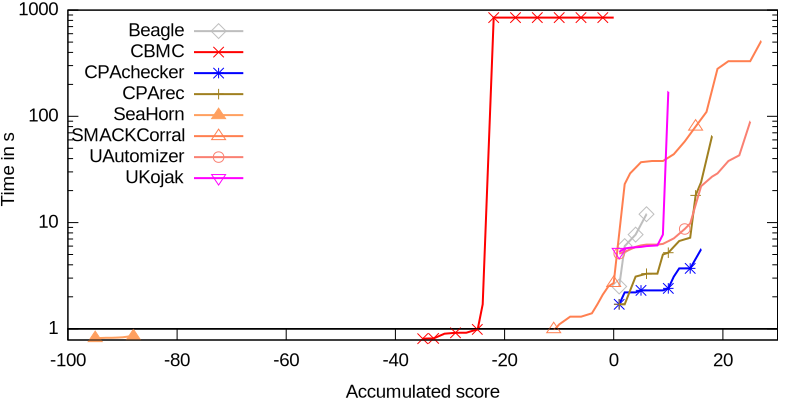
\includegraphics[width=\textwidth]{fig/competition-result}
  \caption{Accumulated Score over Time}
  \label{figure:accumulated-score}
\end{figure}


%%% Local Variables: 
%%% mode: latex
%%% TeX-master: "draft"
%%% LaTeX-command: "latex -shell-escape"
%%% End: 
